\chapter{Experimentální výsledky} \label{chapt:experiments}
Tato kapitola prezentuje výsledky experimentů popsaných v sekci~\ref{sec:experiments-design}. 
Cílem experimentů je vyhodnotit výkonnost jednotlivých kvantově inspirovaných evolučních algoritmů a jejich klasických protějšků. 

Nejprve jsou uvedeny výsledky ladění parametrů pro jednotlivé kvantově inspirovaná evoluční algoritmy. 
Tyto optimalizované parametry jsou následně aplikovány na rozsáhlejší instance problému batohu, jejichž výsledky jsou také prezentovány. 
Každý graf je doplněn o informaci z tabulky~\ref{tab:experiments-design}, která udává optimální hodnotu řešení problému batohu pro jednotlivé velikosti testovaných instancí.

Na základě získaných dat je v závěru kapitoly vedena diskuze porovnávající klasické evoluční algoritmy s jejich kvantově inspirovaným variantami, včetně analýzy jejich silných a slabých stránek. 
Zvláštní pozornost je věnována také vzájemnému srovnání jednotlivých kvantově inspirovaných evolučních algoritmů.

\section{Kvantově inspirovaný genetický algoritmus}\label{sec:exp-qisa}
V této části jsou představeny experimentální výsledky týkající se kvantově inspirovaného genetického algoritmu (\emph{QIGA}). 
Pozornost je věnována zejména vlivu různých hodnot parametru $\Delta\theta$ a velikosti populace na kvalitu nalezených řešení. 

\begin{figure}[ht!]
    \centering
    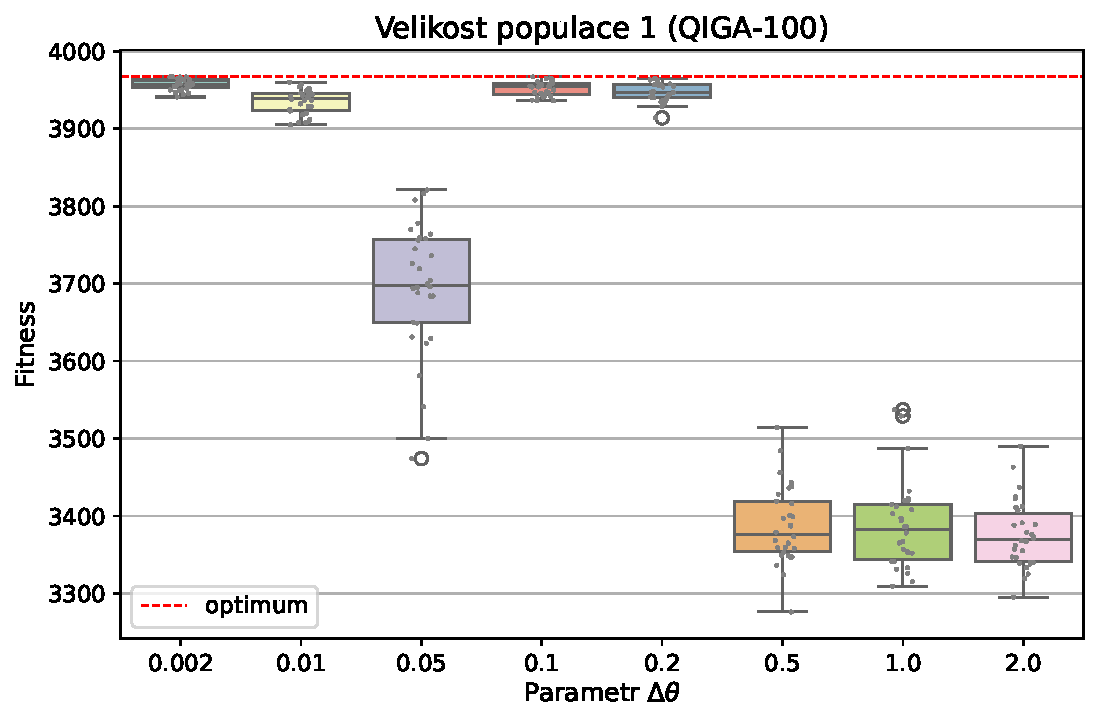
\includegraphics[width=0.7\textwidth]{qiga/boxplot_qiga_100_popsize_1.pdf}
    \caption{Vliv různých hodnot parametru $\Delta\theta$ při velikosti populace 1 a instanci problému se 100 položkami.}
    \label{fig:qiga-pop1}
\end{figure}

Na obrázku~\ref{fig:qiga-pop1} jsou zobrazeny výsledky experimentů pro problém o 100 položkách s~populací tvořenou jediným jedincem.
Sledován je vliv různých hodnot parametru $\Delta\theta$, jejichž konkrétní nastavení vychází z tabulky~\ref{tab:qiga-all-instance}. 
Prezentovány jsou pouze výsledky pro jednoho jedince, neboť algoritmus \emph{QIGA}, jak bylo uvedeno v sekci~\ref{sec:exp-qiga}, neobsahuje mechanismus pro sdílení informací mezi jedinci v populaci. 

Z dat v obrázku~\ref{fig:qiga-pop1} a přehledu statistických charakteristik v tabulce~\ref{tab:qiga-theta-stats} vyplývá, že parametr $\Delta\theta$ má významný vliv na kvalitu řešení. 
Nejlepších řešení bylo dosaženo při $\Delta\theta = 0,002$, kde se průměrná kvalita řešení pohybovala velmi blízko optimu a současně vykazovala nejnižší rozptyl. 

Obecně platí, že nižší hodnoty parametru $\Delta\theta$ vedly k lepším výsledkům s výjimkou anomálie při $\Delta\theta = 0,05$. 
Naopak vyšší hodnoty (zejména od 0,5 a výše) vedly ke znatelnému zhoršení kvality řešení, doprovázené vyšší směrodatnou odchylkou, což naznačuje nižší stabilitu algoritmu. 

Z výsledků lze usuzovat, že vyšší hodnoty $\Delta\theta$ způsobují příliš velkou rotaci kvantového hradla, což má za následek chaotické a méně efektivní prohledávaní prostoru možných řešení. 
\begin{table}[ht]
    \centering
    \begin{tabular}{c c c c c c c}
        \toprule
        \(\Delta\theta\) & Průměr & Směrodatná odchylka & Medián & Q1 & Q3\\
        \midrule
        0,002 & 3\,956,90 & 7,18  & 3\,957 & 3\,952,75 & 3\,963,0  \\
        0,01  & 3\,934,73 & 15,80 & 3\,939 & 3\,923,50 & 3\,945,75 \\
        0,05  & 3\,692,63 & 87,03 & 3\,698 & 3\,649,25 & 3\,757,5  \\
        0,1   & 3\,951,80 & 9,13  & 3\,954 & 3\,944,50 & 3\,957,75 \\
        0,2   & 3\,947,40 & 11,75 & 3\,947 & 3\,940,25 & 3\,956,75 \\
        0,5   & 3\,387,03 & 50,06 & 3\,376 & 3\,354,25 & 3\,418,25 \\
        1,0   & 3\,387,07 & 56,67 & 3\,382 & 3\,343,75 & 3\,414,25 \\
        2,0   & 3\,375,50 & 43,71 & 3\,369 & 3\,341,50 & 3\,403,0  \\
        \bottomrule
    \end{tabular}
    \caption{Statistické charakteristiky výsledků pro různé hodnoty parametru \(\Delta\theta\) (optimální hodnota řešení je 3967).}
    \label{tab:qiga-theta-stats}
\end{table}

Na základě předchozích výsledků byly z dalších experimentů vyřazeny hodnoty parametru $\Delta\theta = 0,5, 1$ a $2$, neboť opakovaně vedly k výrazně horším výsledkům. 
Hodnota $0,05$ však byla ponechána, ačkoliv také nepatřila mezi nejúspěšnější, neboť spadá do oblasti hodnot, které v jiných případech vedly k velmi kvalitním řešením. 
Právě z tohoto důvodu byla tato anomálie zachována i v následujících experimentech, aby mohla být dále analyzována ve vztahu k větším instancím problému. 

Tato anomálie byla dále zkoumána v kontextu různých velikostí populace, respektive v~závislosti na celkovém počtu vyhodnocení fitness funkce. 
Výsledky zobrazené na obrázku~\ref{fig:qiga-100-all} ukazují, že vliv velikosti populace na kvalitu řešení není přímočarý. 
Nejhorší výsledky byly dosaženy při populaci tvoření jediným jedincem. 
Se zvyšujícím se počtem jedinců se však kvalita zlepšovala a nejlepších výsledků bylo dosaženo při desítkách jedinců v populaci. 
Při dalším zvyšování velikosti populace však kvalita opět začala mírně klesat.

Z grafu~\ref{fig:qiga-100-all} je rovněž patrné, že algoritmus dosahoval lepších výsledků při populaci velikosti 5, ve srovnání s jedním jedincem, a to při nastavení parametru $\Delta\theta = 0,02$.  
Tato anomálie může být vysvětlena tím, že i když algoritmus \emph{QIGA} nepodporuje sdílení informací mezi jedinci, větší počet jedinců zvyšuje šanci, že alespoň jeden z nich nalezne kvalitní řešení. 
To je zvlášť pravděpodobné v tomto případě, kdy instance obsahuje 100 položek a~počet evaluací je 10\;000, což poskytuje jednotlivým jedincům dostatek prostoru pro jejich vývoj. 

\begin{figure}[ht!]
    \centering
    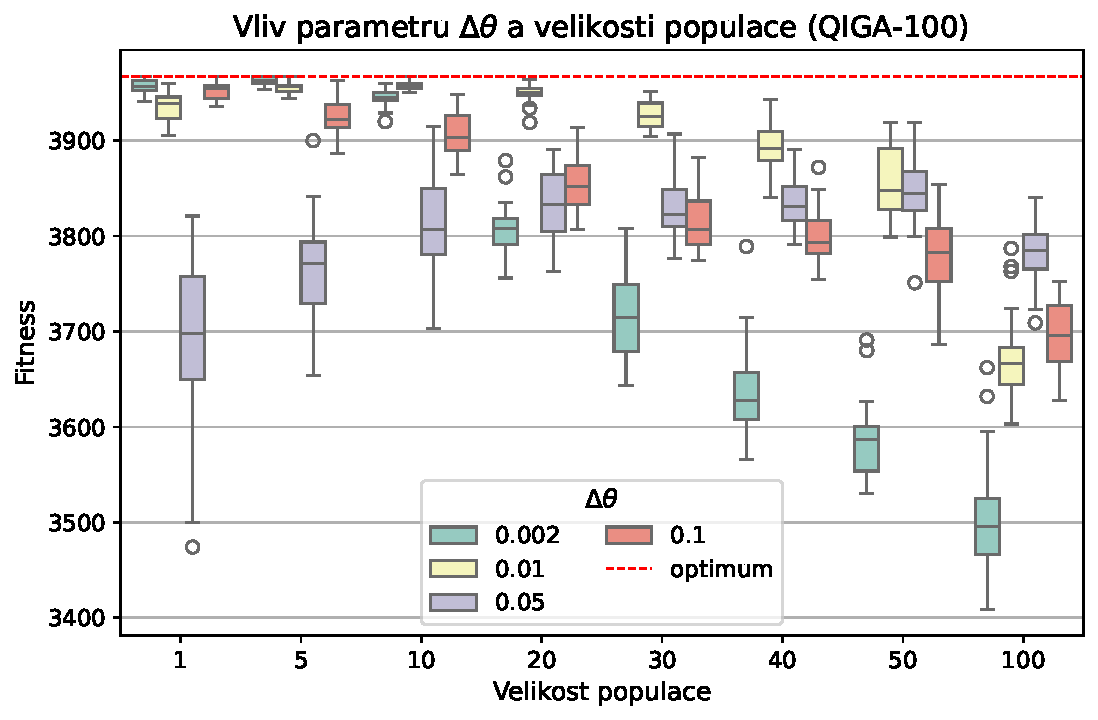
\includegraphics[width=0.98\textwidth]{qiga/boxplot_qiga_100_all_theta.pdf}
    \caption{Závislost kvality řešení na velikosti populace pro různé hodnoty parametru $\Delta\theta$ u instance se 100 položkami.}
    \label{fig:qiga-100-all}
\end{figure}

Toto tvrzení lze ověřit pomocí obrázku~\ref{fig:qiga-500-all}, kde byla velikost instance problému navýšena na 500 položek, zatímco celkový počet evaluací zůstal zachován. 
Z grafu je patrné, že v tomto případě dosahovala nejlepších výsledků populace tvořena pouze jedním jedincem, protože větší populace neměly dostatek prostoru pro rozvoj.

\begin{figure}[ht!]
    \centering
    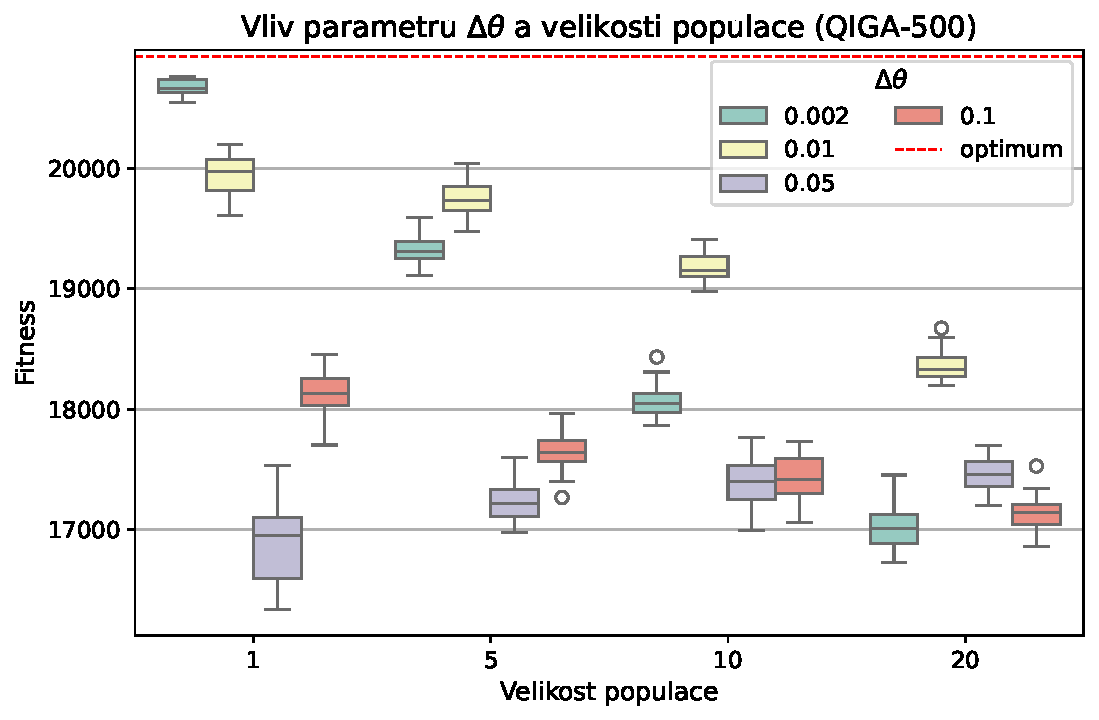
\includegraphics[width=0.98\textwidth]{qiga/boxplot_qiga_500_all_theta.pdf}
    \caption{Závislost kvality řešení na velikosti populace pro různé hodnoty parametru $\Delta\theta$ při instanci 500.}
    \label{fig:qiga-500-all}
\end{figure}

Anomálie pozorovaná při hodnotě parametru $\Delta\theta = 0,005$ lze vysvětlit vlivem zaokrouhlovacích chyb a konvergence, kdy kvantové pravděpodobnosti postupně směřují k hodnotám velmi blízkým nule nebo jedné (např. $0,0000\dots$ nebo $0,9999\dots$). 
V takovém případě se prakticky zastaví změny pozorovaného chromozomu, čímž se výrazně omezí možnost dalšího průzkumu prostoru řešení.  
Naopak při mírně odlišných hodnotách parametru (např. $\Delta\theta = 0,051$) zůstávají pravděpodobnosti méně extrémní (např. $0,0002$ a $0,9998$), což zachovává možnost dalšího zlepšení. 
Podobně jako v předchozím případě se i zde ukázalo, že u~větších instancí problému vedla větší velikost populace k lepším výsledkům, neboť přítomnost více jedinců v populaci zvyšovala šanci na nalezení kvalitnějšího řešení.

Obrázek~\ref{fig:qiga-large} shrnuje výsledky experimentů provedených na rozsáhlejších instancích problému batohu, při doladěné hodnotě parametru $\Delta\theta = 0,002$. 
\begin{figure}[ht!]
    \centering
    \begin{subfigure}[b]{0.24\textwidth}
      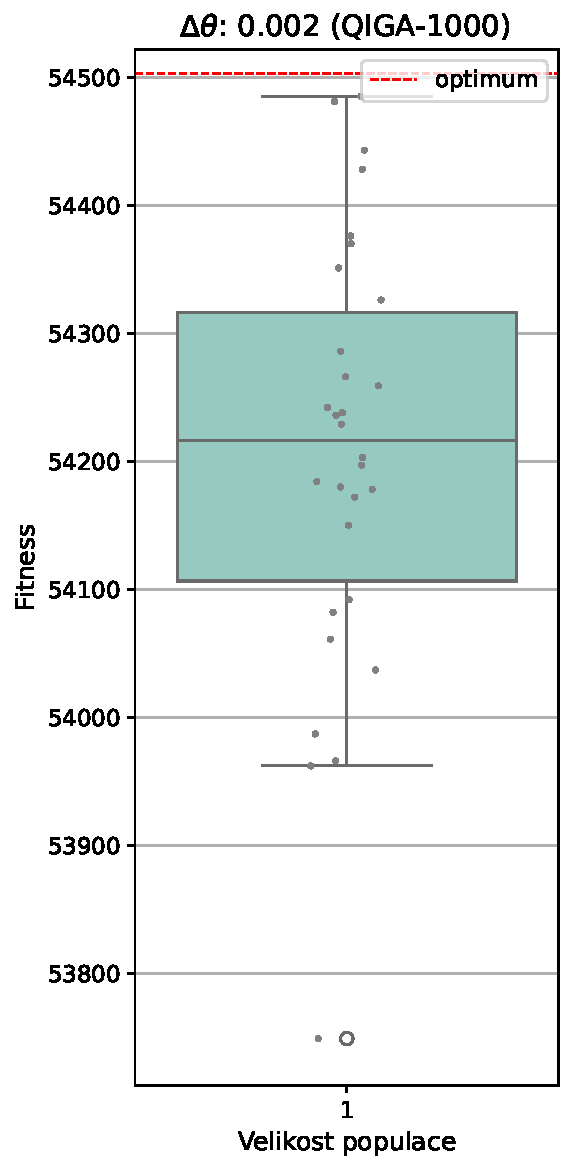
\includegraphics[width=\linewidth]{qiga/boxplot_qiga_1000_theta_0.002.pdf}
    \end{subfigure}
    \hfill
    \begin{subfigure}[b]{0.24\textwidth}
        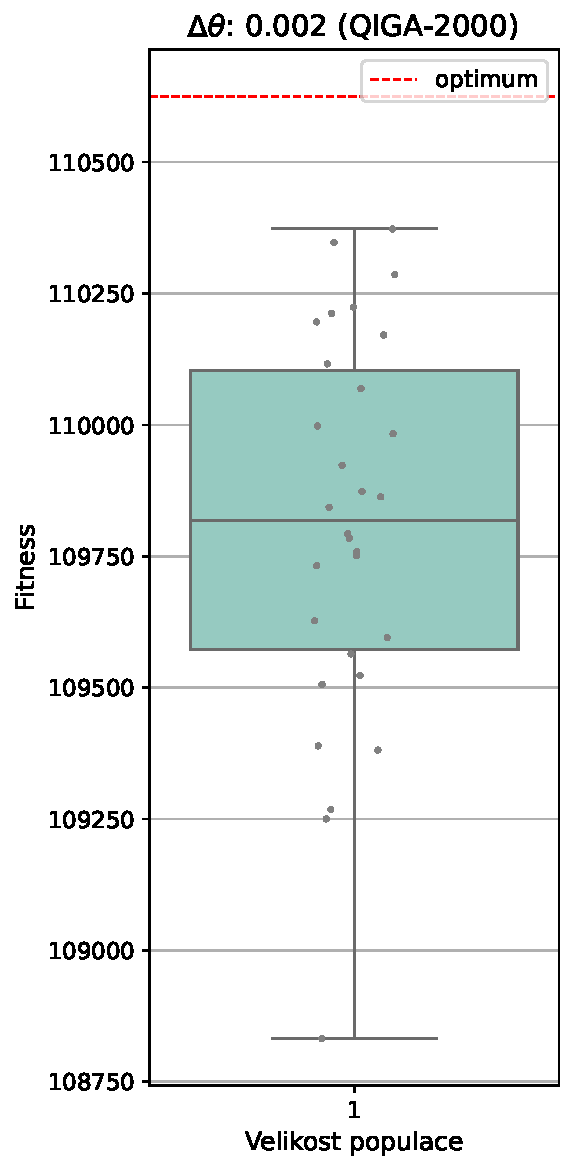
\includegraphics[width=\linewidth]{qiga/boxplot_qiga_2000_theta_0.002.pdf}
    \end{subfigure}
    \hfill
    \begin{subfigure}[b]{0.24\textwidth}
        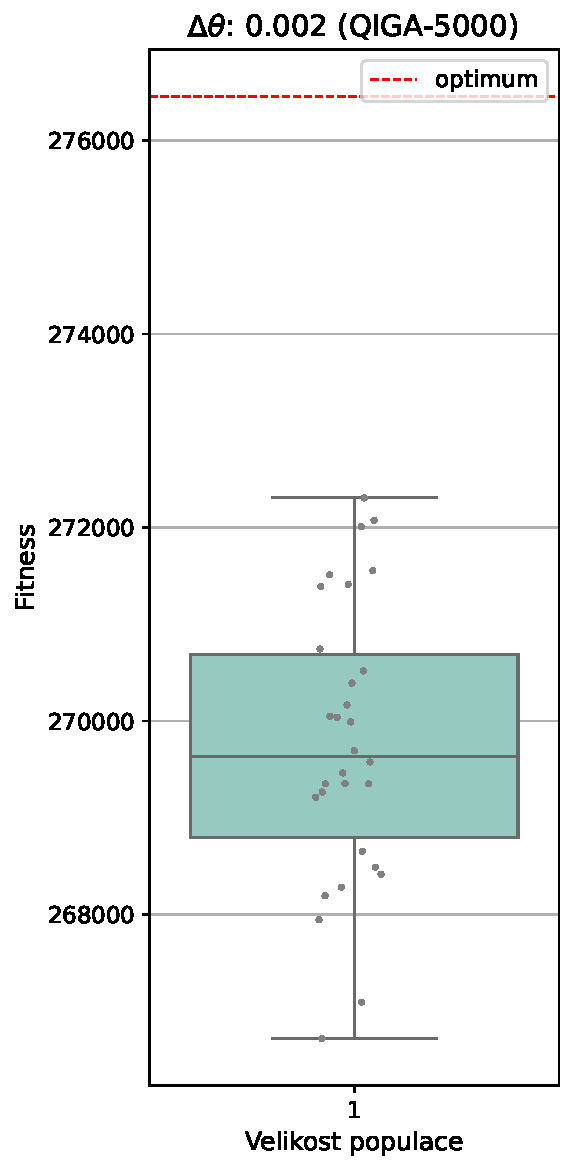
\includegraphics[width=\linewidth]{qiga/boxplot_qiga_5000_theta_0.002.pdf}
    \end{subfigure}
    \hfill
    \begin{subfigure}[b]{0.24\textwidth}
        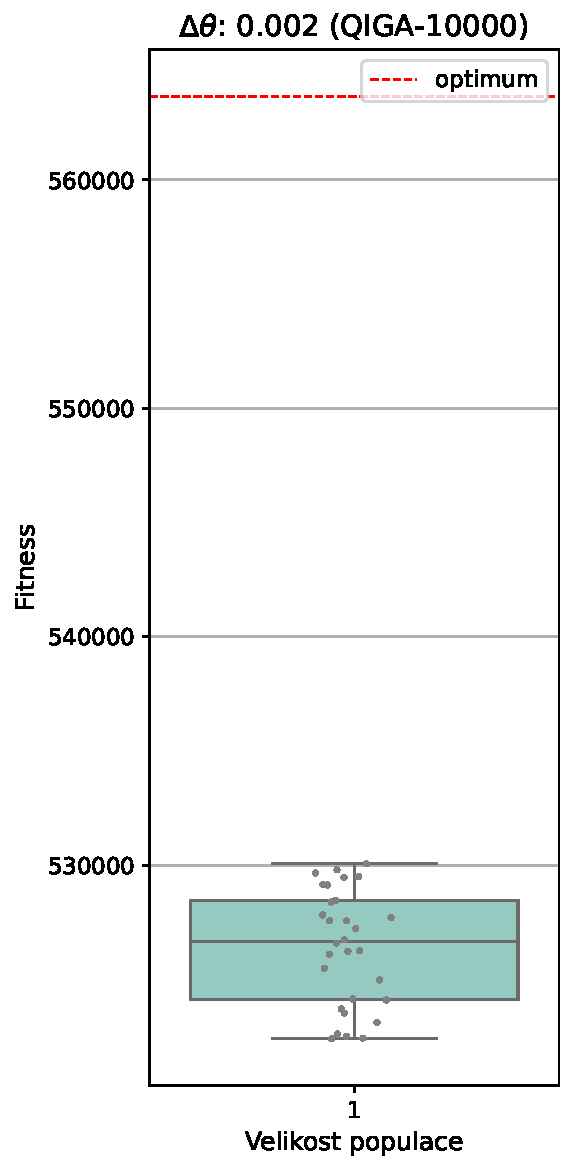
\includegraphics[width=\linewidth]{qiga/boxplot_qiga_10000_theta_0.002.pdf}
    \end{subfigure}
  
    \caption{Porovnání kvality řešení \emph{QIGA} při hodnotě $\Delta\theta = 0,002$ a různých velikostech instance batohu.}
    \label{fig:qiga-large}
\end{figure}

Z výsledků je patrné, že u instancích o velikosti 1\,000 a 2\,000 se algoritmus \emph{QIGA} stále dokáže přiblížit k optimálnímu řešení. 
Naopak u větších instancí, konkrétně 5\,000 a 10\,000, již dochází k poklesu kvality řešení, což lze přičíst omezenému počtu evaluací. 

Obrázek~\ref{fig:qiga-convergence} zachycuje rychlost konvergence při velikostech instancí 500 a 2\,000. 
V obou případech byla použita jednočlenná populace a doladěná hodnota parametru $\Delta\theta = 0,002$.
\begin{figure}[ht!]
    \centering
    \begin{subfigure}[b]{0.48\textwidth}
      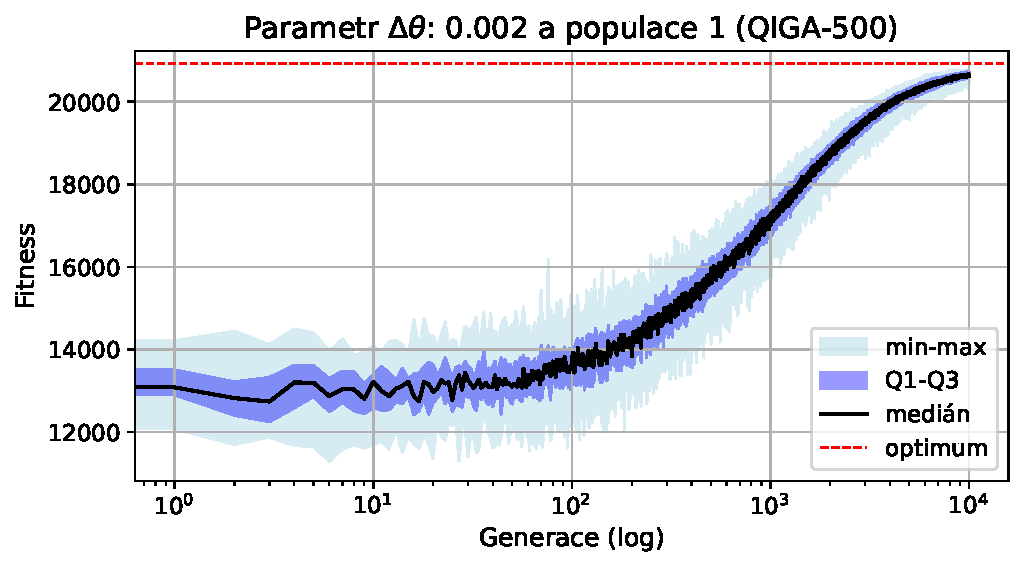
\includegraphics[width=\linewidth]{qiga/qiga_convergence_500_theta_0.002_population_1.pdf}
    \end{subfigure}
    \hfill
    \begin{subfigure}[b]{0.48\textwidth}
        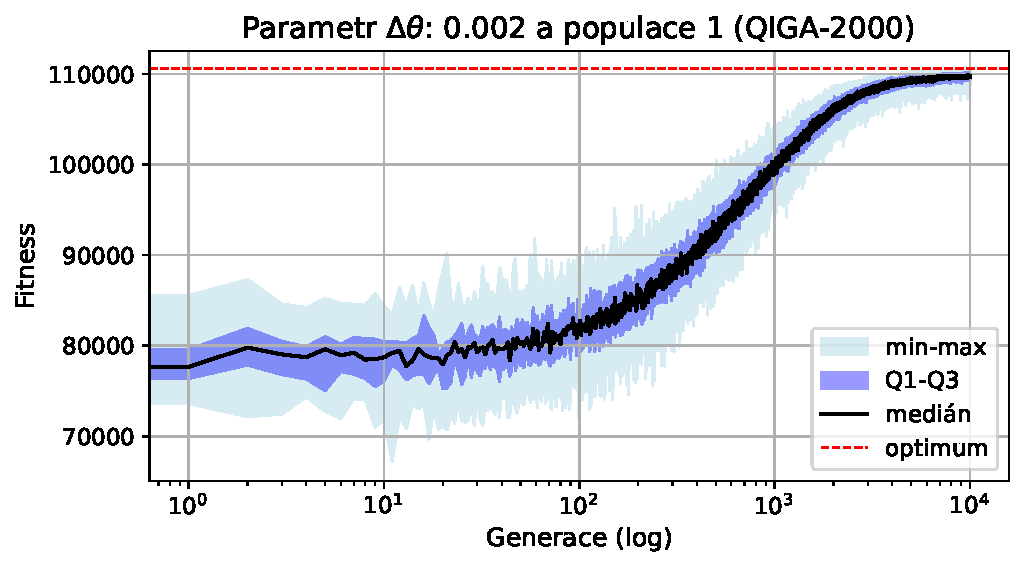
\includegraphics[width=\linewidth]{qiga/qiga_convergence_2000_theta_0.002_population_1.pdf}
    \end{subfigure}
    \caption{Konvergenční křivky pro $\Delta\theta = 0,002$ a velikosti instancí 500 a 2\,000.}
    \label{fig:qiga-convergence}
\end{figure}

\section{Kvantově inspirované simulované žíhání}\label{sec:exp-qiga}
\section{Kvantová evoluce roje}\label{sec:exp-qse}
\section{Kvantově inspirovaná op timalizace rojem částic}\label{sec:exp-qipso}
\section{Klasická varianta GA, SA a PSO}\label{sec:exp-ea}
\section{Porovnání kvantově inspirovaných evolučních algoritmů}
\section{Diskuze výsledků}